\documentclass[tikz]{standalone}

\usepackage{lmodern}

\begin{document}

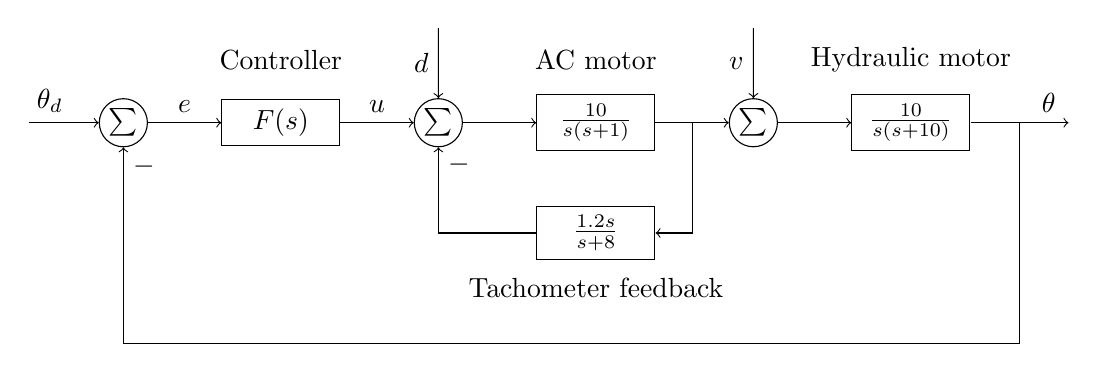
\begin{tikzpicture}[scale = 0.8, node distance=20mm, block/.style={rectangle, draw, minimum width=15mm}, sumnode/.style={circle, draw, inner sep=1pt, font={\fontsize{4pt}{4pt}\selectfont}, scale=1}]
  \node[coordinate] (refinput) {};
  \node[sumnode, right of=refinput, node distance=12mm] (sumerr) {$\sum$};
  \node[block, right of=sumerr, node distance=20mm] (controller) {$F(s)$};
  \node[above of=controller, node distance=8mm] {Controller};
  \node[sumnode, right of=controller, node distance=20mm] (sumcal) {\tiny $\sum$};
  \node[block, right of=sumcal, node distance=20mm] (AC) {$\frac{10}{s(s + 1)}$};
  \node[above of=AC, node distance=8mm] {AC motor};
  \node[block, below of=AC, node distance=14mm] (ACfb) {$\frac{1.2s}{s + 8}$};
  \node[below of=ACfb, node distance=7mm] {Tachometer feedback};

  \node[sumnode, right of=AC, node distance=20mm] (sumdist) {\tiny $\sum$};
  \node[block, right of=sumdist, node distance=20mm] (hydraulic) {$\frac{10}{s(s+10)}$};
  \node[above of=hydraulic, node distance=8mm] {Hydraulic motor};
  \node[coordinate, right of=hydraulic, node distance=20mm] (output) {};

  \node[coordinate, above of=sumcal, node distance=12mm] (caldist) {};
  \node[coordinate, above of=sumdist, node distance=12mm] (winddist) {};

  \draw[->] (hydraulic) -- node[coordinate] (measure) {} node[above, pos=0.8] {$\theta$} (output);

  \draw[->] (refinput) -- node[above, pos=0.3] {$\theta_d$} (sumerr);
  \draw[->] (sumerr) -- node[above] {$e$} (controller);
  \draw[->] (controller) -- node[above] {$u$} (sumcal);
  \draw[->] (sumcal) -- node[above] {$$} (AC);
  \draw[->] (AC) -- node[coordinate] (measureac) {} (sumdist);
  \draw[->] (measureac) |- (ACfb);
  \draw[->] (ACfb) -| node[right, pos=0.9] {$-$} (sumcal);

  \draw[->] (measure) -- ++(0,-35mm) -| node[right, pos=0.95] {$-$} (sumerr);
  \draw[->] (caldist) -- node[left] {$d$} (sumcal);
  \draw[->] (winddist) -- node[left] {$v$} (sumdist);
  \draw[->] (sumdist) -- node[left] {} (hydraulic);
  

\end{tikzpicture}
\end{document}
